\documentclass[11pt,a4paper]{article}
\usepackage[utf8]{inputenc}
\usepackage{amsmath,amssymb,amsfonts}
\usepackage{geometry}
\usepackage{graphicx}
\usepackage{booktabs}
\usepackage{hyperref}
\usepackage{tikz}
\usetikzlibrary{calc, patterns, angles, quotes}

\geometry{top=2.5cm, bottom=2.5cm, left=2.5cm, right=2.5cm}

\title{\textbf{Modellazione Dinamica di un Sistema Carrello-Multi-Link con Carico Rettangolare via Eulero-Lagrange}}
\author{\textbf{Alessandro Prisco} \\ Università degli Studi di Napoli Federico II}
\date{\today}

\begin{document}
	
	\maketitle
	
	\begin{abstract}
		In questa relazione viene derivato il modello dinamico completo a parametri concentrati di un sistema meccanico complesso composto da un carrello lineare privo di attuazione diretta sul primo giunto (giunto passivo), connesso in serie a due bracci rotanti (link) e a un corpo rigido terminale di forma rettangolare. La modellazione viene eseguita applicando rigorosamente il formalismo di Eulero-Lagrange. Il sistema presenta caratteristiche di sottoattuazione e accoppiamenti inerziali non lineari significativi, rendendolo un benchmark ideale per l'analisi dei sistemi multibody e la progettazione di controllori industriali avanzati.
	\end{abstract}
	
	\section{Descrizione del Sistema Meccanico}
	Il sistema in esame è costituito da quattro corpi principali connessi in serie:
	\begin{enumerate}
		\item \textbf{Carrello (Corpo 0):} Di massa $m_0$, con movimento vincolato esclusivamente lungo l'asse orizzontale, identificato dalla coordinata lineare $x$.
		\item \textbf{Primo Link (Corpo 1):} Di massa $m_1$, lunghezza $L_1$ e momento d'inerzia $I_1$ valutato rispetto al proprio centro di massa ($CoM_1$). Esso è connesso al carrello tramite un \textbf{giunto rotoidale passivo}.
		\item \textbf{Secondo Link (Corpo 2):} Di massa $m_2$, lunghezza $L_2$ e momento d'inerzia $I_2$ rispetto al proprio centro di massa ($CoM_2$). Esso è connesso al primo link tramite un \textbf{giunto rotoidale attivo} azionato dalla coppia $\tau_2$.
		\item \textbf{Rettangolo Terminale (Corpo 3):} Di massa $m_3 = m_{\text{rect}}$ e momento d'inerzia $I_3 = I_{\text{rect}}$ rispetto al proprio centro di massa ($CoM_3$). La particolarità geometrica di questo sistema prevede che l'estremità finale del secondo link sia incernierata \textbf{esattamente in corrispondenza del centro di massa} del rettangolo tramite un \textbf{giunto rotoidale attivo} azionato dalla coppia $\tau_3$.
	\end{enumerate}
	
	L'orientamento di ciascun corpo rigido è parametrizzato mediante gli angoli assoluti $\theta_1$, $\theta_2$ e $\theta_3$ definiti rispetto all'orizzontale, come illustrato nello schema cinematico seguente.
	
	\begin{figure}[h!]
		\centering
		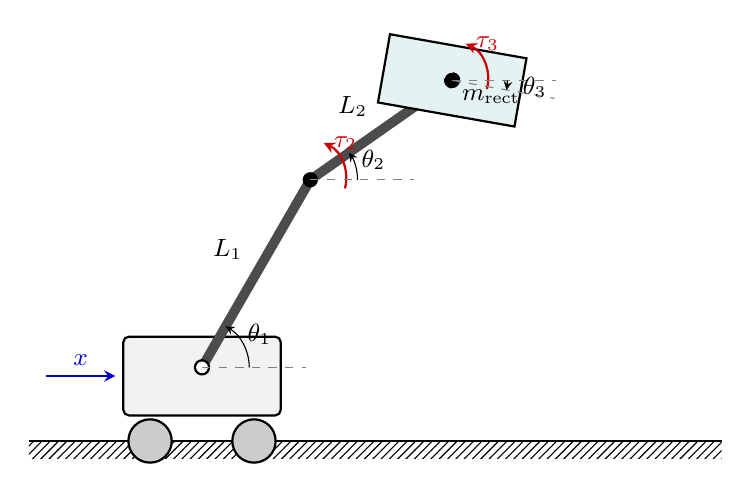
\begin{tikzpicture}[>=stealth, scale=1.1, font=\small]
			% --- Parametri Geometrici ---
			\def\cartW{2.0}
			\def\cartH{1.0}
			\def\wheelR{0.25}
			\def\Lone{2.5}
			\def\Ltwo{2.0}
			\def\rectW{1.6}
			\def\rectH{0.8}
			\def\thetaOne{60}    
			\def\thetaTwo{35}    
			\def\thetaThree{-10} 
			
			% --- Stili ---
			\tikzset{
				cart/.style={draw=black, thick, fill=gray!10, rounded corners=2pt},
				link/.style={draw=black!70, line width=3.5pt, line cap=round},
				passive_joint/.style={circle, draw=black, fill=white, inner sep=1.8pt, thick},
				active_joint/.style={circle, draw=black, fill=black, inner sep=1.8pt},
				ground/.style={pattern=north east lines, draw=none},
				com/.style={circle, draw=black, inner sep=0pt, minimum size=5pt, fill=white, append after command={
						\pgfextra{
							\draw[fill=black] (\tikzlastnode.center) -- ++(0:2.5pt) arc(0:90:2.5pt) -- cycle;
							\draw[fill=black] (\tikzlastnode.center) -- ++(180:2.5pt) arc(180:270:2.5pt) -- cycle;
						}
				}}
			}
			
			% --- Ground ---
			\draw[thick] (-2, -\wheelR) -- (6, -\wheelR);
			\fill[ground] (-2, -\wheelR-0.2) rectangle (6, -\wheelR);
			
			% --- Carrello ---
			\node[cart, minimum width=\cartW cm, minimum height=\cartH cm] (cart) at (0, \cartH/2) {};
			\draw[thick, fill=gray!40] (-0.6, -\wheelR) circle (\wheelR);
			\draw[thick, fill=gray!40] (0.6, -\wheelR) circle (\wheelR);
			\draw[->, thick, blue!80!black] (-1.8, \cartH/2) -- (-1.0, \cartH/2) node[above, midway] {$x$};
			
			% --- Coordinate Giunti ---
			\coordinate (J1) at (0, \cartH/2 + 0.1); 
			\coordinate (J2) at ($(J1) + (\thetaOne:\Lone)$);
			\coordinate (J3) at ($(J2) + (\thetaTwo:\Ltwo)$);
			
			% --- Links ---
			\draw[link] (J1) -- (J2) node[midway, above left, text=black] {$L_1$};
			\draw[link] (J2) -- (J3) node[midway, above left, text=black] {$L_2$};
			
			% --- Rettangolo Terminale ---
			\begin{scope}[shift={(J3)}, rotate=\thetaThree]
				\draw[thick, fill=teal!10] (-\rectW/2, -\rectH/2) rectangle (\rectW/2, \rectH/2);
				\node[com] (com_rect) at (0,0) {};
				\node[below right] at (0,0) {$m_{\text{rect}}$};
			\end{scope}
			
			% --- Giunti ---
			\node[passive_joint] at (J1) {};
			\node[active_joint] at (J2) {};
			\draw[->, thick, red!80!black] ($(J2)+(0.4, -0.1)$) arc (-15:65:0.45) node[right] {$\tau_2$};
			\node[active_joint] at (J3) {};
			\draw[->, thick, red!80!black] ($(J3)+(0.4, -0.1)$) arc (-15:65:0.45) node[right] {$\tau_3$};
			
			% --- Riferimenti Angolari ---
			\draw[dashed, gray] (J1) -- ++(1.2, 0) coordinate (ref1);
			\draw[dashed, gray] (J2) -- ++(1.2, 0) coordinate (ref2);
			\draw[dashed, gray] (J3) -- ++(1.2, 0) coordinate (ref3);
			
			\pic [draw, ->, "$\theta_1$", angle eccentricity=1.4, angle radius=0.6cm] {angle = ref1--J1--J2};
			\pic [draw, ->, "$\theta_2$", angle eccentricity=1.4, angle radius=0.6cm] {angle = ref2--J2--J3};
			
			\coordinate (rect_edge) at ($(J3) + (\thetaThree:1.2)$);
			\draw[dashed, gray] (J3) -- (rect_edge);
			\pic [draw, <-, "$\theta_3$", angle eccentricity=1.5, angle radius=0.7cm] {angle = rect_edge--J3--ref3};
		\end{tikzpicture}
		\caption{Schema cinematico e convenzioni della meccanica applicate al robot.}
		\label{fig:schema_robot}
	\end{figure}
	
	\section{Cinematica dei Centri di Massa}
	Definiamo il vettore delle coordinate generalizzate come:
	\begin{equation}
		q = \begin{bmatrix} x \\ \theta_1 \\ \theta_2 \\ \theta_3 \end{bmatrix} \in \mathbb{R}^4
	\end{equation}
	
	Assumendo che i link siano barre omogenee, la posizione cartesiana dei centri di massa ($p_{ci}$) e del rettangolo terminale ($p_{c3}$) in un sistema di riferimento fisso con origine sulla guida del carrello è definita da:
	\begin{align}
		p_{c0} &= \begin{bmatrix} x \\ 0 \end{bmatrix} \\
		p_{c1} &= \begin{bmatrix} x + \frac{L_1}{2}\cos\theta_1 \\ \frac{L_1}{2}\sin\theta_1 \end{bmatrix} \\
		p_{c2} &= \begin{bmatrix} x + L_1\cos\theta_1 + \frac{L_2}{2}\cos\theta_2 \\ L_1\sin\theta_1 + \frac{L_2}{2}\sin\theta_2 \end{bmatrix} \\
		p_{c3} &= \begin{bmatrix} x + L_1\cos\theta_1 + L_2\cos\theta_2 \\ L_1\sin\theta_1 + L_2\sin\theta_2 \end{bmatrix}
	\end{align}
	
	Derivando rispetto al tempo, otteniamo i vettori velocità lineari di ciascun centro di massa:
	\begin{align}
		v_{c0} &= \begin{bmatrix} \dot{x} \\ 0 \end{bmatrix} \\
		v_{c1} &= \begin{bmatrix} \dot{x} - \frac{L_1}{2}\sin\theta_1 \dot{\theta}_1 \\ \frac{L_1}{2}\cos\theta_1 \dot{\theta}_1 \end{bmatrix} \\
		v_{c2} &= \begin{bmatrix} \dot{x} - L_1\sin\theta_1 \dot{\theta}_1 - \frac{L_2}{2}\sin\theta_2 \dot{\theta}_2 \\ L_1\cos\theta_1 \dot{\theta}_1 + \frac{L_2}{2}\cos\theta_2 \dot{\theta}_2 \end{bmatrix} \\
		v_{c3} &= \begin{bmatrix} \dot{x} - L_1\sin\theta_1 \dot{\theta}_1 - L_2\sin\theta_2 \dot{\theta}_2 \\ L_1\cos\theta_1 \dot{\theta}_1 + L_2\cos\theta_2 \dot{\theta}_2 \end{bmatrix}
	\end{align}
	
	I quadrati dei moduli delle velocità lineari, fondamentali per il calcolo dell'energia cinetica, risultano:
	\begin{align}
		\|v_{c0}\|^2 &= \dot{x}^2 \\
		\|v_{c1}\|^2 &= \dot{x}^2 + \frac{L_1^2}{4}\dot{\theta}_1^2 - L_1\sin\theta_1 \dot{x}\dot{\theta}_1 \\
		\|v_{c2}\|^2 &= \dot{x}^2 + L_1^2\dot{\theta}_1^2 + \frac{L_2^2}{4}\dot{\theta}_2^2 - 2L_1\sin\theta_1 \dot{x}\dot{\theta}_1 - L_2\sin\theta_2 \dot{x}\dot{\theta}_2 + L_1 L_2\cos(\theta_1-\theta_2)\dot{\theta}_1\dot{\theta}_2 \\
		\label{eq:v3_sq} \|v_{c3}\|^2 &= \dot{x}^2 + L_1^2\dot{\theta}_1^2 + L_2^2\dot{\theta}_2^2 - 2L_1\sin\theta_1 \dot{x}\dot{\theta}_1 - 2L_2\sin\theta_2 \dot{x}\dot{\theta}_2 + 2L_1 L_2\cos(\theta_1-\theta_2)\dot{\theta}_1\dot{\theta}_2
	\end{align}
	
	\section{Formulazione Energetica e Lagrangiana}
	L'energia cinetica totale del sistema $T(q, \dot{q})$ è data dalla somma dell'energia cinetica lineare e rotazionale di ciascun corpo:
	\begin{equation}
		T = \frac{1}{2}m_0 \|v_{c0}\|^2 + \sum_{i=1}^3 \left( \frac{1}{2}m_i \|v_{ci}\|^2 + \frac{1}{2}I_{i}\dot{\theta}_i^2 \right)
	\end{equation}
	
	Sostituendo le espressioni cinematiche precedentemente ricavate, l'energia cinetica totale si scrive come:
	\begin{align}
		T = & \frac{1}{2}(m_0 + m_1 + m_2 + m_3)\dot{x}^2 \nonumber\\
		& + \frac{1}{2}\left(I_1 + \frac{1}{4}m_1 L_1^2 + m_2 L_1^2 + m_3 L_1^2\right)\dot{\theta}_1^2 \nonumber\\
		& + \frac{1}{2}\left(I_2 + \frac{1}{4}m_2 L_2^2 + m_3 L_2^2\right)\dot{\theta}_2^2 + \frac{1}{2}I_3\dot{\theta}_3^2 \nonumber\\
		& - \left(\frac{1}{2}m_1 + m_2 + m_3\right)L_1\sin\theta_1 \dot{x}\dot{\theta}_1 - \left(\frac{1}{2}m_2 + m_3\right)L_2\sin\theta_2 \dot{x}\dot{\theta}_2 \nonumber\\
		& + \left(\frac{1}{2}m_2 + m_3\right)L_1 L_2\cos(\theta_1-\theta_2)\dot{\theta}_1\dot{\theta}_2
	\end{align}
	
	L'energia potenziale totale $V(q)$, considerando l'accelerazione di gravità $g$ agente lungo la verticale negativa, è dovuta unicamente alle quote dei centri di massa dei link e del rettangolo:
	\begin{equation}
		V = m_1 g \left(\frac{L_1}{2}\sin\theta_1\right) + m_2 g \left(L_1\sin\theta_1 + \frac{L_2}{2}\sin\theta_2\right) + m_3 g \left(L_1\sin\theta_1 + L_2\sin\theta_2\right)
	\end{equation}
	Raggruppando i termini costanti, otteniamo:
	\begin{equation}
		V = \left(\frac{1}{2}m_1 + m_2 + m_3\right)gL_1\sin\theta_1 + \left(\frac{1}{2}m_2 + m_3\right)gL_2\sin\theta_2
	\end{equation}
	
	La funzione Lagrangiana $\mathcal{L}(q, \dot{q})$ è definita come:
	\begin{equation}
		\mathcal{L} = T - V
	\end{equation}
	
	\section{Equazioni del Moto}
	Le equazioni dinamiche si ricavano applicando le equazioni di Eulero-Lagrange per ciascuna coordinata generalizzata $q_i$:
	\begin{equation}
		\frac{d}{dt}\left(\frac{\partial \mathcal{L}}{\partial \dot{q}_i}\right) - \frac{\partial \mathcal{L}}{\partial q_i} = Q_i, \quad i=1,\dots,4
	\end{equation}
	dove $Q_i$ rappresenta la forza o coppia generalizzata associata alla coordinata $q_i$.
	
	\subsection{Lavoro Virtuale e Forze Generalizzate}
	I giunti attivi applicano coppie relative. Sia un'eventuale forza esterna $F$ agente sul carrello lungo l'asse $x$. Le coppie attuatrici $\tau_2$ e $\tau_3$ agiscono rispettivamente sulle variazioni relative degli angoli $(\theta_2 - \theta_1)$ e $(\theta_3 - \theta_2)$. Il lavoro virtuale $\delta W$ del sistema è espresso da:
	\begin{equation}
		\delta W = F\delta x + \tau_2(\delta\theta_2 - \delta\theta_1) + \tau_3(\delta\theta_3 - \delta\theta_2)
	\end{equation}
	Riorganizzando i termini rispetto alle variazioni delle coordinate assolute $\delta q$, si ottiene:
	\begin{equation}
		\delta W = F\delta x - \tau_2\delta\theta_1 + (\tau_2 - \tau_3)\delta\theta_2 + \tau_3\delta\theta_3
	\end{equation}
	Il vettore delle forze generalizzate risulta quindi:
	\begin{equation}
		Q = \begin{bmatrix} Q_x \\ Q_{\theta_1} \\ Q_{\theta_2} \\ Q_{\theta_3} \end{bmatrix} = \begin{bmatrix} F \\ -\tau_2 \\ \tau_2 - \tau_3 \\ \tau_3 \end{bmatrix}
	\end{equation}
	
	\subsection{Forma Matriciale Standard}
	Sviluppando le derivate parziali, il modello dinamico può essere espresso nella classica forma matriciale compatta dello spazio dei giunti:
	\begin{equation}\label{eq:matrix_form}
		M(q)\ddot{q} + C(q, \dot{q})\dot{q} + G(q) = Q
	\end{equation}
	
	Per semplificare la scrittura delle matrici, si definiscono le seguenti tre costanti raggruppate, che racchiudono le proprietà inerziali e geometriche combinate della catena cinematica:
	\begin{align}
		K_1 &= \left(\frac{1}{2}m_1 + m_2 + m_3\right)L_1 \\
		K_2 &= \left(\frac{1}{2}m_2 + m_3\right)L_2 \\
		K_3 &= \left(\frac{1}{2}m_2 + m_3\right)L_1 L_2
	\end{align}
	
	\subsubsection{Matrice d'Inerzia $M(q)$}
	La matrice di massa $M(q) \in \mathbb{R}^{4 \times 4}$ è simmetrica e definita positiva:
	\begin{equation}
		M(q) = \begin{bmatrix}
			M_{11} & -K_1\sin\theta_1 & -K_2\sin\theta_2 & 0 \\
			-K_1\sin\theta_1 & M_{22} & K_3\cos(\theta_1-\theta_2) & 0 \\
			-K_2\sin\theta_2 & K_3\cos(\theta_1-\theta_2) & M_{33} & 0 \\
			0 & 0 & 0 & I_3
		\end{bmatrix}
	\end{equation}
	dove i termini diagonali principali sono costanti e pari a:
	\begin{align}
		M_{11} &= m_0 + m_1 + m_2 + m_3 \\
		M_{22} &= I_1 + \left(\frac{1}{4}m_1 + m_2 + m_3\right)L_1^2 \\
		M_{33} &= I_2 + \left(\frac{1}{4}m_2 + m_3\right)L_2^2
	\end{align}
	
	Si noti come la quarta riga e colonna, relative alla dinamica rotazionale del rettangolo attorno al proprio $CoM$, risultino completamente disaccoppiate dal punto di vista inerziale diretto, in quanto il giunto risiede esattamente nel baricentro del rettangolo.
	
	\subsubsection{Matrice di Coriolis e Forze Centrifughe $C(q, \dot{q})$}
	La matrice dei termini centripeti e di Coriolis $C(q, \dot{q}) \in \mathbb{R}^{4 \times 4}$ è formulata in modo tale da soddisfare la proprietà di emisimmetria della matrice $(\dot{M} - 2C)$, utile per le analisi di stabilità di Lyapunov:
	\begin{equation}
		C(q, \dot{q}) = \begin{bmatrix}
			0 & -K_1\cos\theta_1 \dot{\theta}_1 & -K_2\cos\theta_2 \dot{\theta}_2 & 0 \\
			0 & 0 & K_3\sin(\theta_1-\theta_2)\dot{\theta}_2 & 0 \\
			0 & -K_3\sin(\theta_1-\theta_2)\dot{\theta}_1 & 0 & 0 \\
			0 & 0 & 0 & 0
		\end{bmatrix}
	\end{equation}
	
	\subsubsection{Vettore di Gravità $G(q)$}
	Il vettore delle forze gravitazionali $G(q) \in \mathbb{R}^4$ si ottiene derivando l'energia potenziale rispetto alle coordinate spaziali:
	\begin{equation}
		G(q) = \frac{\partial V}{\partial q} = \begin{bmatrix}
			0 \\
			K_1 g \cos\theta_1 \\
			K_2 g \cos\theta_2 \\
			0
		\end{bmatrix}
	\end{equation}
	
	\section{Considerazioni sulla Simulazione nello Spazio di Stato}
	Per implementare il modello all'interno di ambienti di simulazione numerica, le equazioni differenziali del secondo ordine del moto \eqref{eq:matrix_form} devono essere esplicitate rispetto alle accelerazioni generalizzate mediante l'inversione della matrice di massa:
	\begin{equation}
		\ddot{q} = M(q)^{-1} \Big( Q - C(q, \dot{q})\dot{q} - G(q) \Big)
	\end{equation}
	
	Definendo il vettore di stato $x_s = \begin{bmatrix} q^T & \dot{q}^T \end{bmatrix}^T \in \mathbb{R}^8$, il sistema dinamico può essere infine riscritto nella classica forma non lineare dello spazio di stato del primo ordine:
	\begin{equation}
		\dot{x}_s = \begin{bmatrix} \dot{q} \\ M(q)^{-1} \Big( Q - C(q, \dot{q})\dot{q} - G(q) \Big) \end{bmatrix}
	\end{equation}
	
	Questo modello esprime accuratamente l'interazione dinamica ed è pronto per essere adoperato sia per scopi di sintesi di leggi di controllo (es. \textit{Feedback Linearization}) sia per l'addestramento tramite algoritmi di Reinforcement Learning.
	
\end{document}